
 \documentclass[acmtog, authorversion]{acmart}
\AtBeginDocument{%
  \providecommand\BibTeX{{%
    \normalfont B\kern-0.5em{\scshape i\kern-0.25em b}\kern-0.8em\TeX}}}
    
\usepackage{algorithm}
\usepackage{amsmath}
\usepackage[noend]{algpseudocode}
\usepackage{subfig}
\renewcommand{\thesubfigure}{Figure \arabic{subfigure}}
\captionsetup[subfigure]{labelformat=simple, labelsep=colon}
\acmYear{2023}
\acmDOI{XXXXXXX.XXXXXXX}
\begin{document}
\fancyfoot{}


\title{Implicit Incompressible SPH}
\author{Jonas BERGER}
\affiliation{%
  \institution{Institut Polytechnique de Paris}
  \country{France}
}


\renewcommand{\shortauthors}{Jonas Berger}

\begin{abstract}
\end{abstract}



%% A "teaser" image appears between the author and affiliation
%% information and the body of the document, and typically spans the
%% page.

%% \begin{teaserfigure}
%%  \centering
%%{\includegraphics[width=\linewidth, height=4cm]{example-image-a}\label{teaser}}
%%  \caption{Caption here}
%%  \label{fig:teaser}
%%\end{teaserfigure}

%%
%% This command processes the author and affiliation and title
%% information and builds the first part of the formatted document.
\maketitle
\thispagestyle{empty}
\section{Introduction}

\begin{figure}
    \centering
    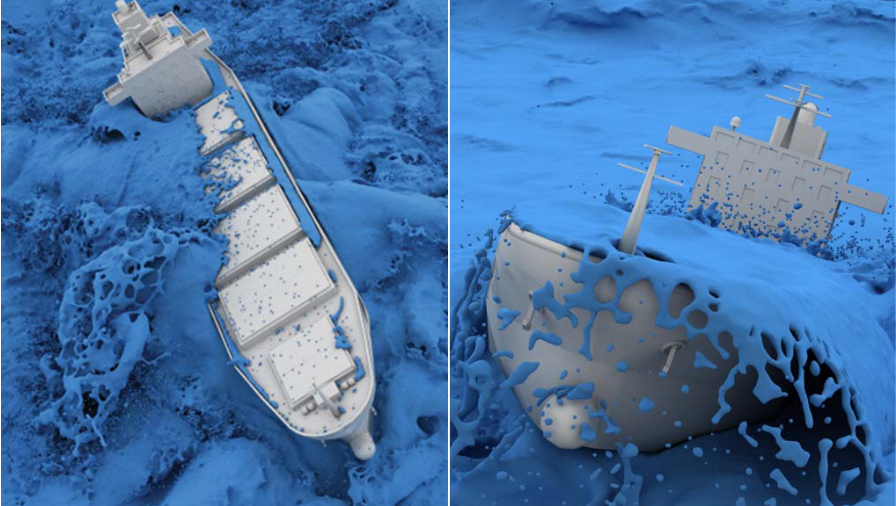
\includegraphics[width=\linewidth]{article_rendering.png}
    \caption{Simulation of IISPH with up to 30 million particles. The picture is taken from \cite{IISPH}.}
    \label{fig:IISPH_article}
\end{figure}

In this report, we will analyze the IISPH method, which is a variant of the famous SPH fluid simulation method.
We will detail the math behind its modelization, see how to implement it, and observe the quantitative and qualitative improvements and flaws of this method over SPH.
The article used for implementing IISPH is \cite{IISPH}. This report is mostly an analysis of what is written in it.

\section{Related works}

The SPH \cite{SPH} is the basis of a lot of different fluid simulation methods. It is quite simple to implement and offers a lot of variants for specific cases such as weakly compressible fluids (WCSPH) \cite{WCSPH} or simply for improvements, such as Predictive-Corrective Incompressible SPH (PCISPH) \cite{PCISPH}.
It relies on an equation of states giving expressions of density, pressure, and different forces according to the position and velocity of particles. One of its main issue is that it doesn't take into account the incompressibility approximation of liquids.
Some articles addresses this issue by creating incompressible SPH, like \cite{PCISPH}, \cite{ISPH} or \cite{ISPHbis}, but faces important performance issues due to the number of equations that such restriction implies and the efficiency of the solver.
The IISPH article \cite{IISPH} proposes an alternative with a model that does not explicitely constraint the density, but will rather induces particles to converge their density to a standard one.
The method proves to be a lot more efficient than the previous ones, and has a satisfying rendering improvement compared to SPH.

\section{Method modelization}

The fluid mecanic is based on a few general equations, some of which serve as the basis for the expressions of the method.
The first one is the continuity equation, derived from the conservation of mass: $\frac{D\rho}{Dt} = -\rho\nabla \cdot \textbf{v}$.
Using the SPH model, we have a detailed expression of the divergence of the velocity: $\nabla \cdot \textbf{v}_{i} = -\frac{1}{\rho_{i}}\sum_{j}m_{j}\textbf{v}_{ij}\nabla W_{ij}$, with $W$ the kernel function and $\textbf{v}_{ij} = \textbf{v}_{i} - \textbf{v}_{j}$.
We deduce from discretization the following relation between density and velocity:

\begin{equation}\label{densityEq}
  \frac{\rho_{i}(t+\Delta t) - \rho_{i}(t)}{\Delta t} = \sum_{j}m_{j}\textbf{v}_{ij}(t+\Delta t)\nabla W_{ij}(t)
\end{equation}

Note that we use the velocity at time $t + \Delta t$ because we wants to constraint the pressure forces, and by \eqref{newtonEq} it implies constraining $\textbf{v}_{ij}(t+\Delta t)$.

The second equation is the incompressibility of the fluid, which implies $\frac{d\rho}{dt} = 0$.
The main idea of the IISPH method is to put this condition indirectly into the equations by searching a state where $\rho_{i}(t+\Delta t) = \rho_{0}$ with $\rho_{0}$ the rest density.

We will consider the three forces in action during the process:


\begin{flalign}
  \text{Gravity: } & \textbf{F}_{i}^{g} = m_{i}\textbf{g} \label{gravityForce}\\
  \text{Viscosity\footnote: } & \textbf{F}_{i}^{v} = 2\nu m_{i}\sum_{j}\frac{m_{j}}{\rho_{j}}\textbf{v}_{ij}\frac{\textbf{x}_{ij}\cdot \nabla W_{ij}}{\textbf{x}_{ij}\cdot\textbf{x}_{ij} + 0.01h^{2}}\\
  \text{Pressure force: } & \textbf{F}_{i}^{p} = -m_{i}\sum_{j}m_{j}\left( \frac{p_{i}}{\rho_{i}^{2}} + \frac{p_{j}}{\rho_{j}^{2}}\right)\nabla W_{ij} \label{pressureEq}
\end{flalign}

\footnotetext{Here, $h$ is the kernel's smoothing length.}
Given the discretization of Newton's second law 

\begin{equation}\label{newtonEq}
  \textbf{v}_{i}(t+\Delta t) = \textbf{v}_{i}(t) + \frac{\Delta t}{m_{i}}\sum \textbf{F}_{i}(t)
\end{equation}
we now have a complete set of equations of state.
The aim here is to mix those equations in order to have a system of equations with the pressures $p_{i}(t)$ as variables.
In order to do this, we will consider gravity and viscosity forces, which do not take pressure into account, and use them into \eqref{newtonEq} and \eqref{densityEq} to express two coefficients who can already be computed: the intermediate velocity and the intermediate density respectively.

\begin{flalign}
   \textbf{v}_{i}^{int} & = \textbf{v}_{i}(t) + \Delta t\frac{\textbf{F}_{i}^{g}(t)+\textbf{F}_{i}^{v}(t)}{m_{i}}\\
   \rho_{i}^{int} & = \rho_{i}(t) + \Delta t \sum_{j}m_{j}\textbf{v}_{ij}^{int}\nabla W_{ij}(t)
\end{flalign}

We can then deduct from \eqref{densityEq} the following equations:

\begin{equation} \label{SOEone}
  \rho_{0} - \rho_{i}^{int} = \Delta t^{2}\sum_{j}m_{j}\left( \frac{\textbf{F}_{i}^{p}(t)}{m_{i}} - \frac{\textbf{F}_{j}^{p}(t)}{m_{j}} \right)\nabla W_{ij}(t)
\end{equation}

In order to make the next equations easier to read and to compute, we will introduce a few other coefficients:

\begin{flalign}
  \textbf{d}_{ij} & = -\Delta t^{2}\frac{m_{j}}{\rho_{j}^{2}} \nabla W_{ij} \text{ for } i \neq j \label{d_ij}\\
  \textbf{d}_{ii} & = -\Delta t^{2}\sum_{j}\frac{m_{i}}{\rho_{i}^{2}} \nabla W_{ij} \label{d_ii}\\
  a_{ij} & = \sum_{k \neq i, j}m_k \left( \textbf{d}_{ij} - \textbf{d}_{kj} \right)\cdot \nabla W_{ik}\\
  \textbf{c}_{i} & = \sum_{j \neq i}\textbf{d}_{ij}p_j
\end{flalign}

Now let's see where to use those new tools.
First of all, notice that by putting \eqref{d_ij} and \eqref{d_ii} into \eqref{pressureEq}, we have $\Delta t^2 \frac{\textbf{F}_i^p}{m_i} = \textbf{d}_{ii}p_i + \sum_{j}\textbf{d}_{ij}p_j$.
Then by putting this expression into \eqref{SOEone}, we have $\rho_{0} - \rho_{i}^{int} = \sum_{j}m_{j}\left( \textbf{d}_{ii}p_i + \sum_{k \neq i}\textbf{d}_{ik}p_k - \textbf{d}_{jj}p_j - \sum_{k \neq j}\textbf{d}_{jk}p_k \right) \cdot \nabla W_{ij}(t)$, which can then be rearranged and simplified into:

\begin{equation} \label{SOEtwo}
  \rho_{0} - \rho_{i}^{int} = \sum_{j}a_{ij}p_j
\end{equation}

Though we finally have a rather simple system of equations in theory, we must address the issue of implementing a solver for such a huge system, and even of storing all those coefficients. Keep in mind the $\textbf{c}_i$, it will soon be used.

\section{Resolution and implementation}

Luckily, we won't have to store, or even to compute, all those coefficients; the two matrix of quadratic dimension would represent too much useless informations.
The article proposes to use the weighted Jacobi method in order to solve \eqref{SOEtwo}.\\
For an equation $A\textbf{x} = \textbf{b}$ with $A$ a diagonally dominant matrix, we can decompose $A = D + N$ with $D$ containing only the diagonal composants of $A$.
Then, we define an arbitrary vector $\textbf{x}^{(0)}$ and the sequence : $\textbf{x}^{(l+1)} = (1 - \omega) \textbf{x}^{(l)} + \omega D^{-1}\left( b - N \textbf{x}^{(l)} \right)$, for $\omega$ between $0$ and $1$.
Not only does the sequence converge to a vector \textbf{x}, but this vector is also solution of the initial equation\footnote{The matrix being diagonally dominant is not a necessary condition for convergence, but it is a sufficient one, and is generally the reason why we use Jacobi method. Especially, the weighted Jacobi method ensures convergence for any matrix when $\omega$ is small enough.}.

In our case, even if we cannot prove that $A$ is diagonally dominant, the implementation shows that the weighted Jacobi method converges rather quickly (cf. next part). The equation here is:

\begin{equation}
  p_i^{l+1} = (1 - \omega) p_i^{n} + \omega \frac{\rho_0 - \rho_i^{int} - \sum_{j \neq i}a_{ij}p_j^l}{a_{ii}}
\end{equation} 

Note that in the case where $a_{ii}$ is zero, then the particle doesn't have any neighbor, and so its pressure must be zero too.\\
For implementation, we can replace that equation with a new one, using the $\textbf{c}_i$ coefficients.

\begin{equation}
  \begin{aligned}
    p_i^{l+1} = & (1 - \omega) p_i^{n} + \omega \frac{1}{a_{ii}}\Bigg( \rho_0 - \rho_i^{int} \\
     - & \sum_{j} m_j \left( \textbf{c}_i - \textbf{c}_j + \textbf{d}_{ji}p_i^l - \textbf{d}_{jj}p_j^l \right)\cdot \nabla W_{ij} \Bigg)
  \end{aligned}
\end{equation}

With this, the implementation becomes pretty straightforward, though with a lot of coefficients to compute: at each time step, we first compute $\rho_i(t)$, $\textbf{v}_{i}^{int}$, $\rho_i^{int}$, $\textbf{d}_{ii}$ and $a_{ii}$.
Then, we iterate the sequence of the weighted Jacobi method : we initiate $p_i^0$, and at each iteration, we compute $\textbf{c}_{i}^{l}$ (notice the exponant, as it now depend on the iteration's pressure) and $p_i^{l+1}$.
After convergence, we can use equations \eqref{gravityForce} through \eqref{newtonEq} to compute velocity, and then position of the particles.

Note that in order to avoid errors in the pressure forces, we need to clamp any negative pressure at each iteration to 0.
The article mentions that an attractive pressure force might be interpreted as surface tension, but is too important in practice, and therefore must be avoided.

\begin{figure}
  \centering
  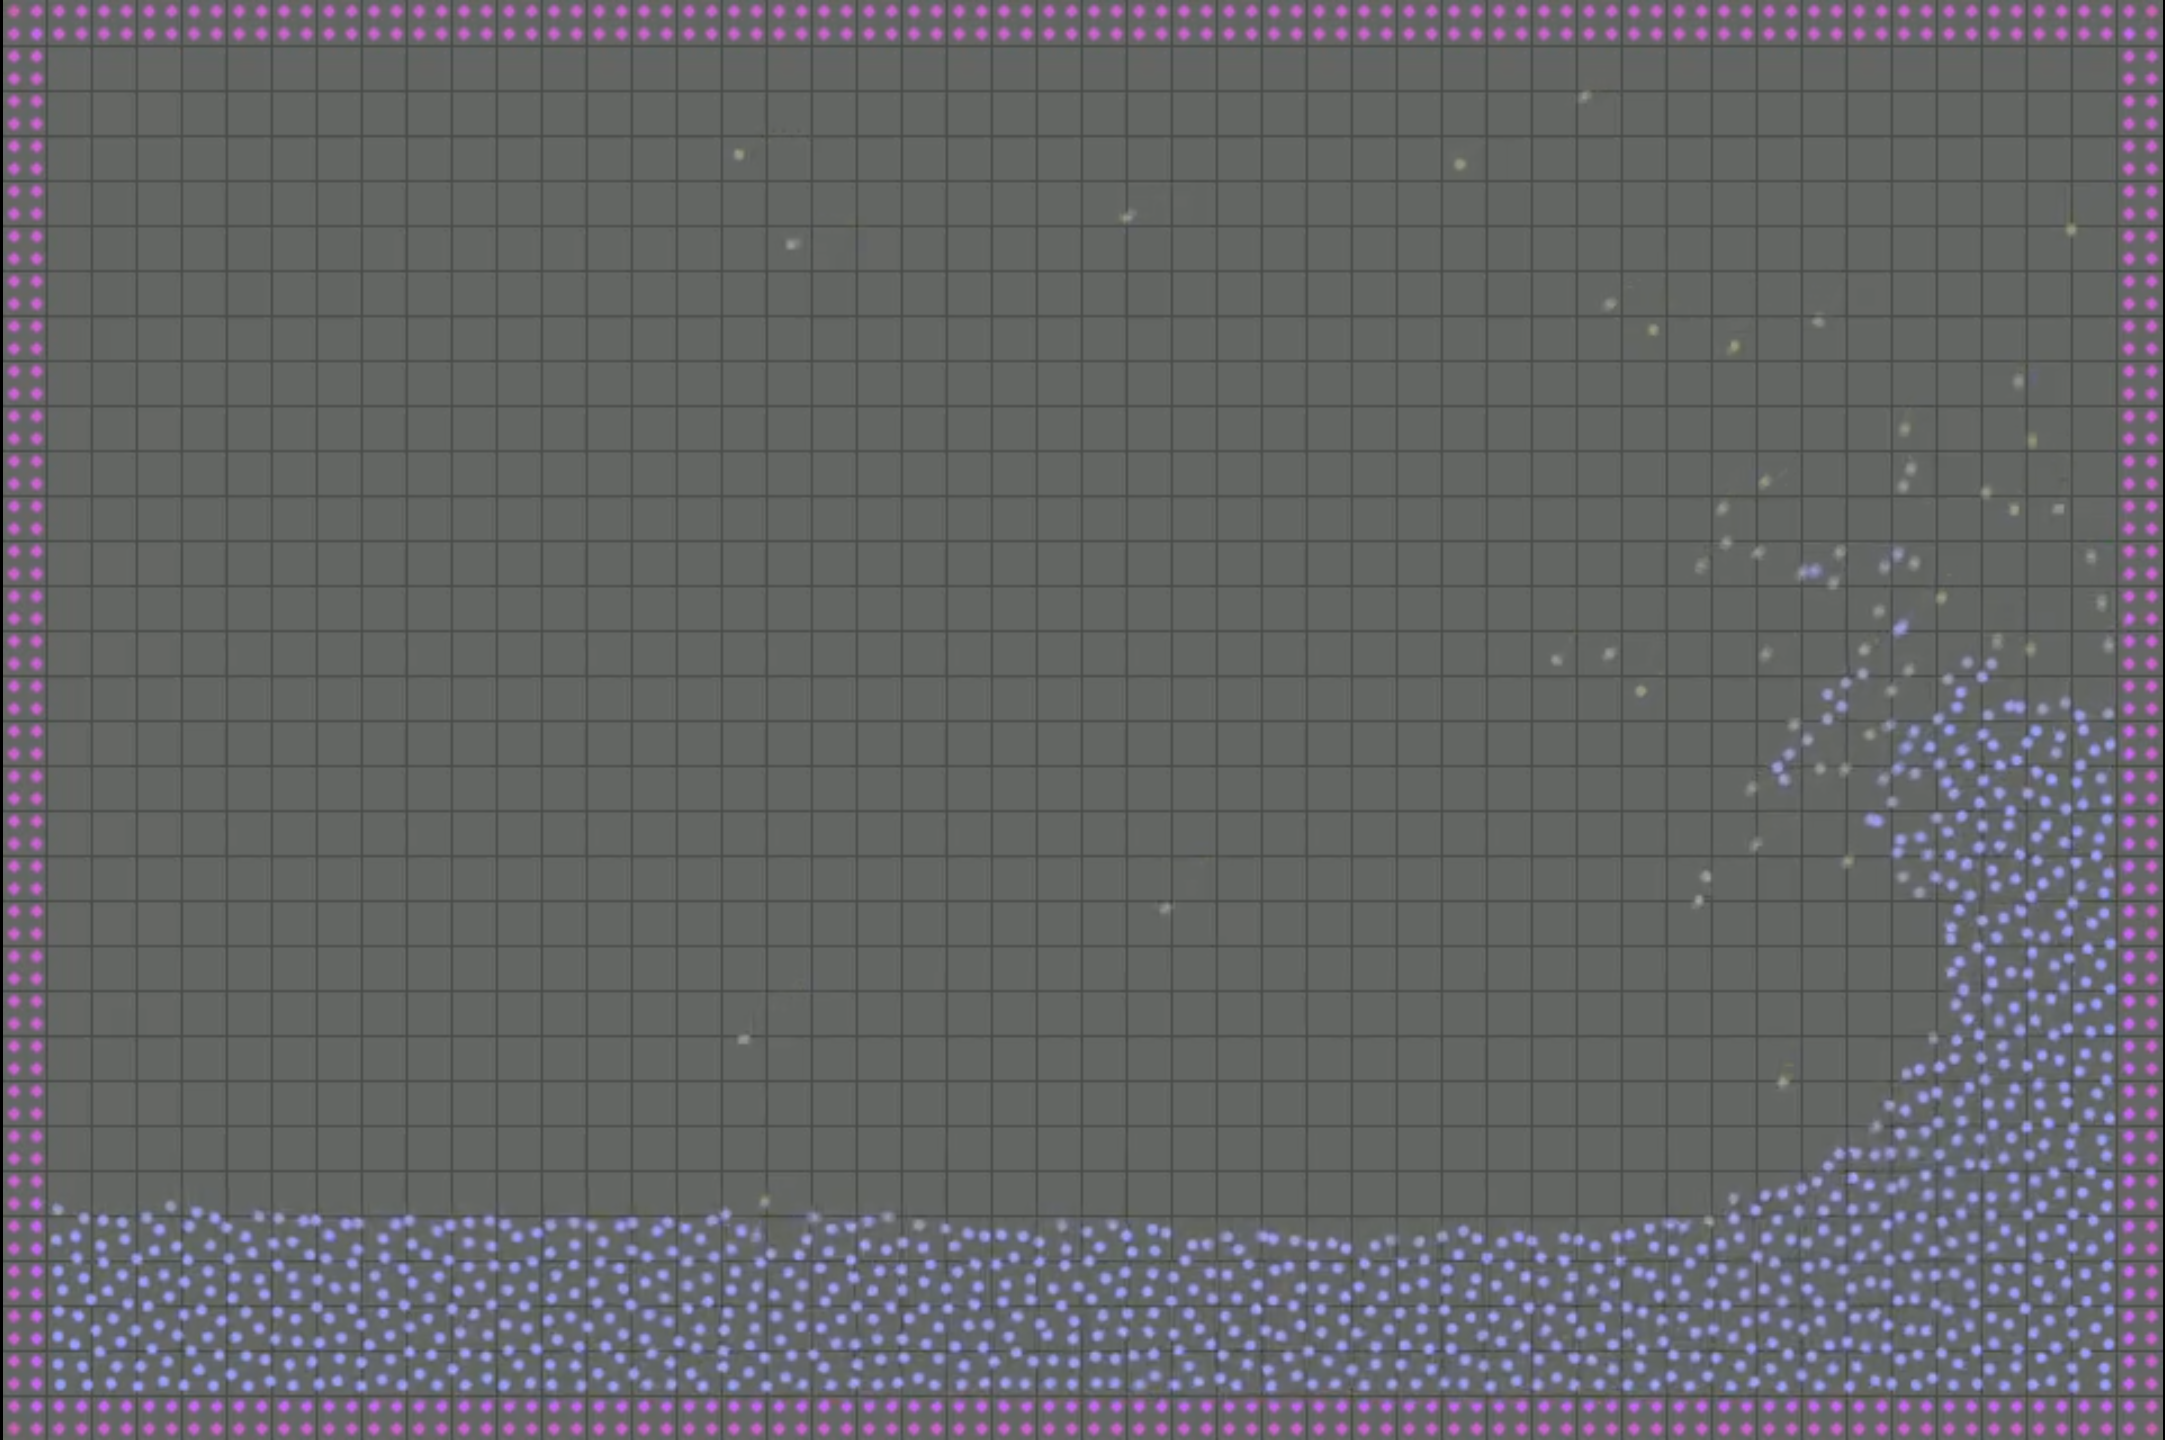
\includegraphics[width=\linewidth]{Wave.png}
  \caption{Simulation of IISPH  \cite{IISPH}.}
  \label{fig:IISPH_first_implementation}
\end{figure}

\section{Optimizations of the method}

The article \cite{IISPH} is a bit unclear about the way to decide the number of iterations of the weighted Jacobi method.
Its stopping criteria is written $\rho_{avg}^l - \rho_0 \le \eta$, with eta an arbitrary constant, and with a minimum of two iterations.
Though we do not compute any density during the iterations, it may be interpreted as $-\frac{1}{N}\sum_{i,j}a_{ij}p_j \le \eta$ with $N$ the number of particle.

There are three issues with this criteria. The first one is the amount of operations to compute just for this number. The algorithm specifically avoid computing every coefficient $a_{ij}$, so a simpler expression is still to be found.
The second one is that this criteria ignore the situation where the density is inferior to the rest density $\rho_0$, which may directly happen at first iteration and not specifically desirable. It can just be resolved by computing the absolute expression.
The final issue is that the criteria is unrelated with the convergence of the system of equations. Having a mean density approximately equal to the rest density doesn't mean that the pressures computed are corrects; in fact, they might be completely random.

In order to avoid this, it might be more important to focus on the variation of pressure between two iterations. By choosing a norm, we can use a criteria of the form $\left\| \textbf{p}^{l+1} - \textbf{p}^l \right\| < \eta$.
There are a lot of ways to compute this, for instance with an $l_2$ norm. We chose one that is quick to compute, that is:

\begin{equation}
  \text{For all i, } \left| p_i^{l+1} - p_i^l \right| < \eta p_i^l
\end{equation}

This criteria observes the relative variation of pressure, and handle well transitions between zero and non-zero pressure. Especially, it ensures that the final pressures are of the right order of magnitude.
The $\eta$ defines the precision we want on the computation. As a good compromise between computation time and precision, we used $\eta = 1$ in our simulation.

The coefficient $\omega$ is a compromise between assured convergence (small value) and fast convergence (value near 1). However, an high $\omega$ does not assure a fast computation, because 1) it may mathematically not converge, or on wrong values,
and 2) it will increase the pressure variations between two iterations. So for a same stopping criteria, an higher $\omega$ will require more iterations to reduce this difference. The article choose a value of $0.5$ by default, and after a few test, it seems that it is the best choice for reducing the number of iterations.
With those numbers, the loop iterates between around 5 and 20 times per time step.

The initialization of $\textbf{p}^0$ does not have a real impact on the performance of the algorithm, as the pressure computed is roughly the same after a few step.
We reused the idea of the article, that is, computing $\textbf{p}^0 = \alpha\textbf{p}(t - \Delta t)$.
After trying a few different values between 0 and 1, there is no apparent difference, except for $\alpha = 0$ which seems to increase considerably the number of iterations.
For the simulation, we simply chose $\alpha = 0.5$.

\begin{figure}
  \centering
  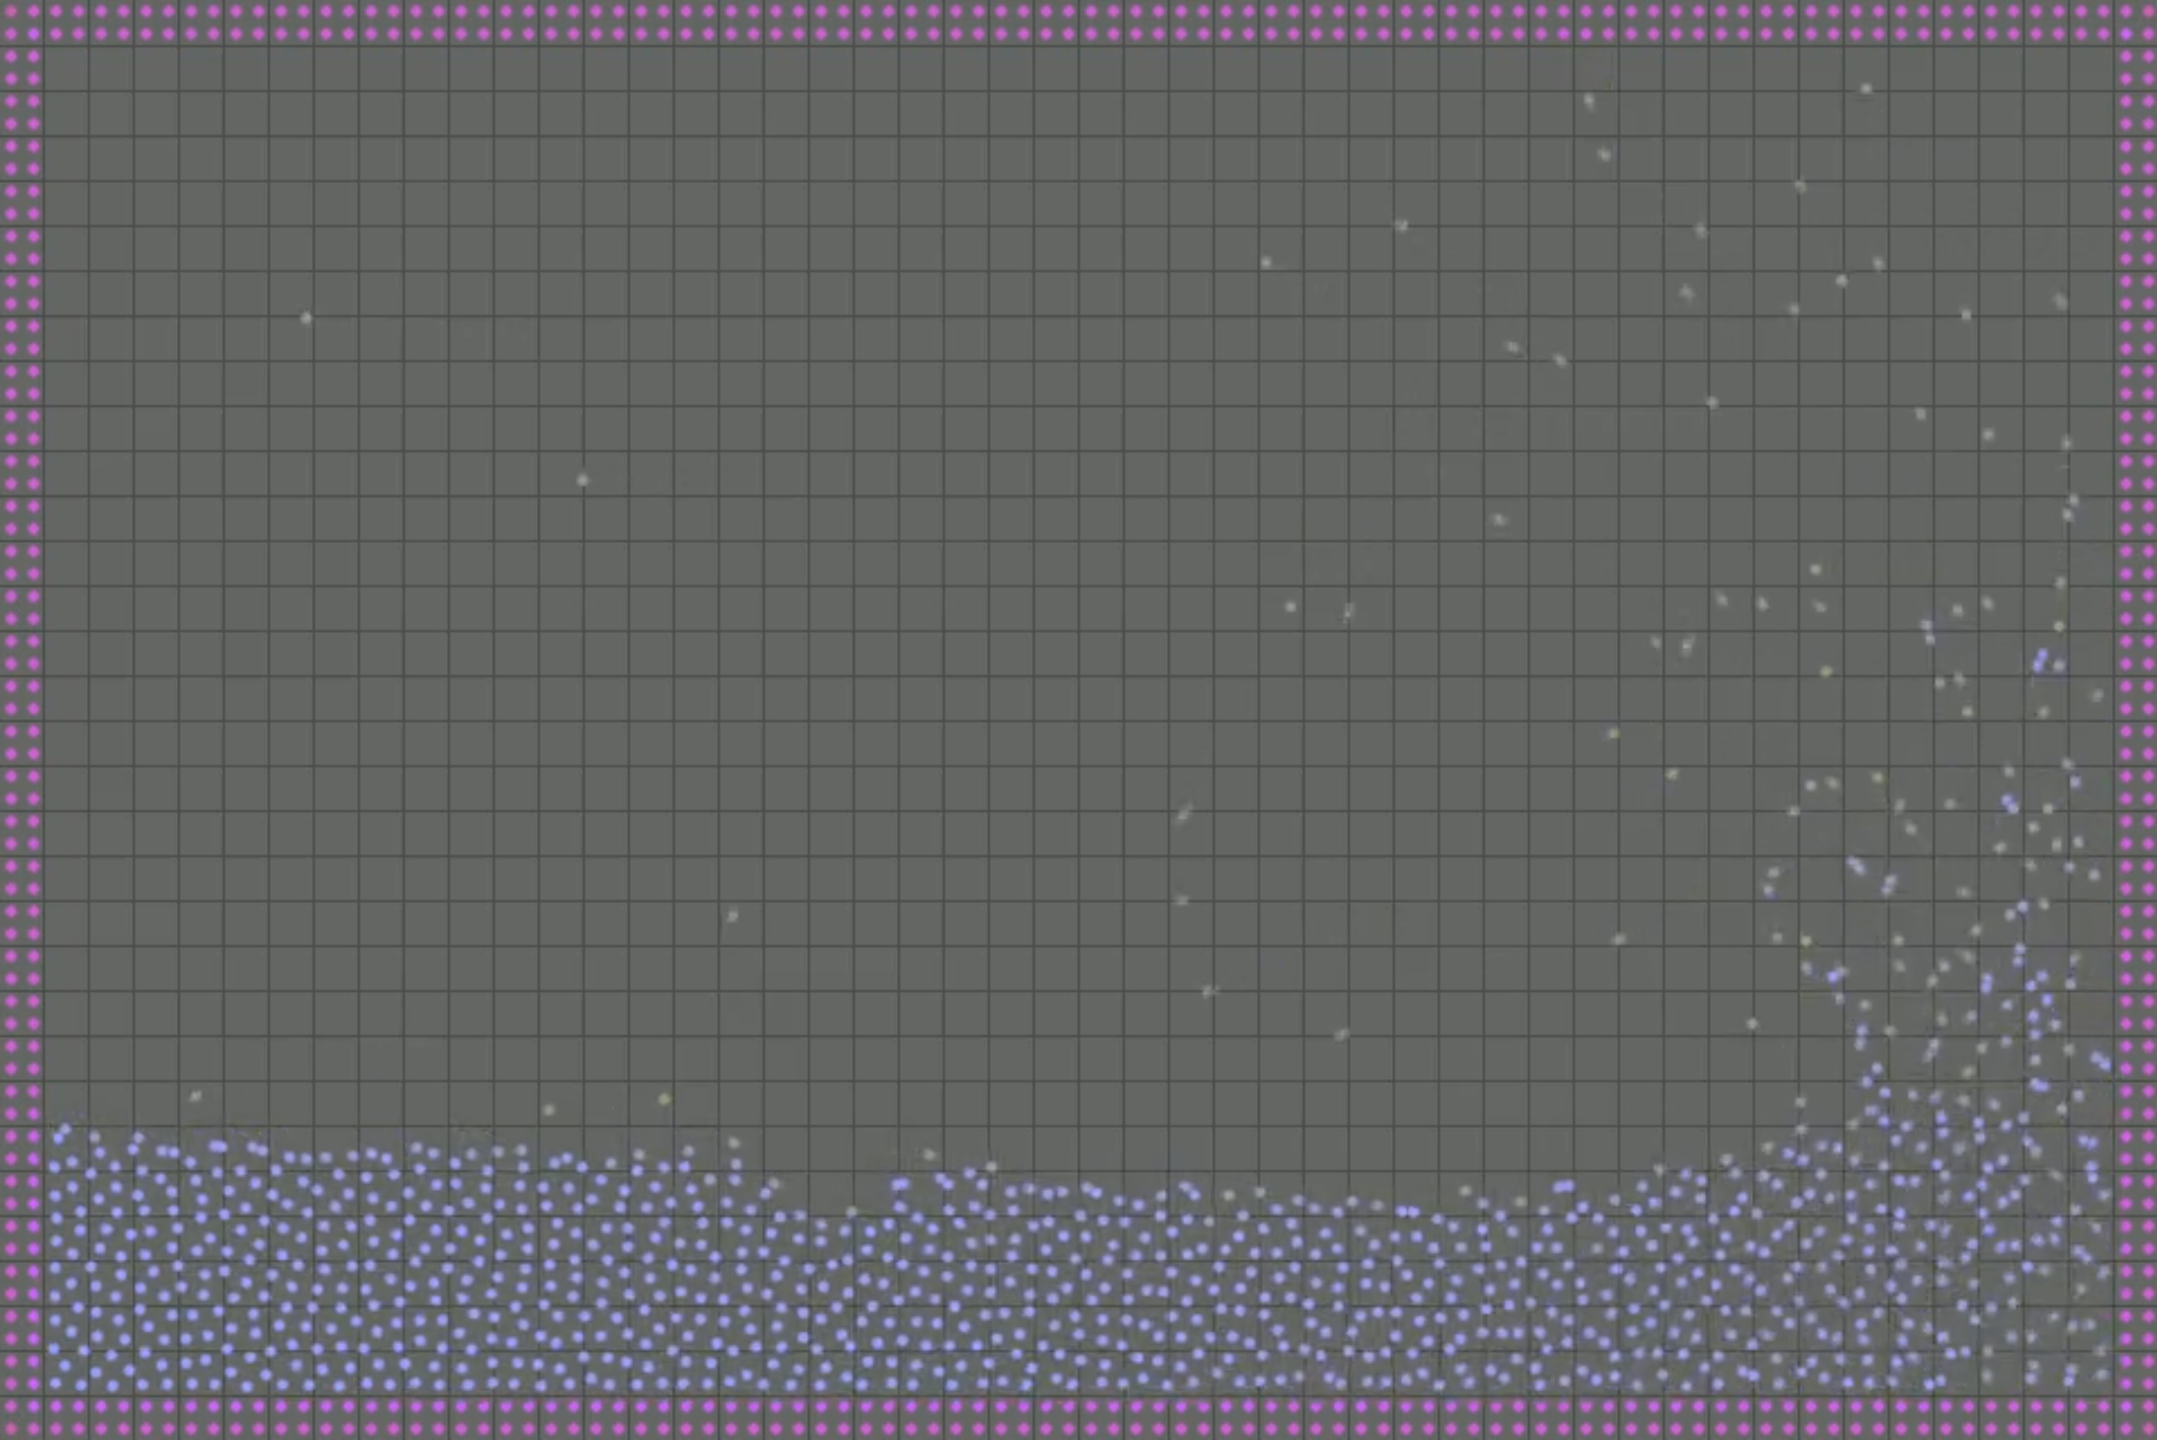
\includegraphics[width=\linewidth]{SPH_wave.png}
  \caption{Implementation of the SPH model \cite{SPH}.}
  \label{fig:SPH}
\end{figure}

Finally, as mentioned in the article, there are no specific boundary handling needed for the IISPH method.
I used a basic one, using stationary particles as walls and using them in the previous equations but imposing their velocity to always be zero.

The article mentioned an implementation of a method from \cite{boundary}, which is rather similar.
Basically, for wall particles, the mass is replaced by a density-dependant one : $\Psi_b(\rho_0) = \frac{\rho_0}{\sum_{b'}W_{bb'}}$, and the pressure is zero, making the pressure force exerced on a fluid particle:

\begin{equation}
  \textbf{F}_{i\gets b}^p = -m_i\Psi_b(\rho_0)\frac{p_i}{\rho_i^2} \nabla W_{ij}
\end{equation}

The mass term is basically a variant of the initial one. A second, compromise implementation between the basic model and this one has been tried (cf. fig. \ref{fig:boundary}) where $\textbf{c}_b$ and $p_b$ are imposed to be zero for the wall particles but the mass is the same as fluid particles (a fixed value).
The iteration for the weighted Jacobi method thus becomes:

\begin{equation}
  \begin{aligned}
    p_i^{l+1} = & (1 - \omega) p_i^{n} + \omega \frac{1}{a_{ii}}\Bigg( \rho_0 - \rho_i^{int} \\
     - & \sum_{j} m_j \left( \textbf{c}_i - \textbf{c}_j + \textbf{d}_{ji}p_i^l - \textbf{d}_{jj}p_j^l \right)\cdot \nabla W_{ij} \\
- & \sum_{b}m_b\textbf{c}_i\cdot \nabla W_{ib}\Bigg)
  \end{aligned}
\end{equation}

\section{Observations}

The simulations were done using a 12-threads 6-core 2.70GHz Intel I5-11400H with 16GB of RAM, and adapt a base code from an SPH implementation in a 2D grid.
For each of them, a frame is drawn every 10 time steps, and we fixed $\Delta t = 0.5ms$. Note that the algorithm has a linear complexity in the number of particles and is adapted for parallelization.

The first test (cf. fig. \ref{fig:IISPH_first_implementation}) was done with a block of 1024 particles and walls composed of 624 stationary particles, for a total of 1648 particles, and as much equations in \eqref{SOEtwo}.
It took 16 minutes and 32 seconds to compute 3000 frames, which means that the algorithm computes one time step every 33ms.
At 60fps, one second of video is computed in 19.86s.\\

For comparison, a similar test was done using the classic SPH method (cf. fig. \ref{fig:SPH}).
It took 2 minutes and 28 seconds for the same number of time steps, which represents 4.9ms to compute one time step, 2.96s to compute one second of video.
The IISPH algorithm thus is about 6.7 times longer.
However, those numbers depend on the context of the simulation, as the weighted Jacobi method have a variable number of iterations, depending on the complexity of the particles arrangement (as mentioned before, roughly between 5 and 20 times).\\

On a qualitative point of view, the IISPH method greatly improves the behaviour of the liquid. It draws smoother shapes, due to a kind of adhesion effect between the particles, created by the implicit incompressibility.
Especially, we can notice a wave effect, with ebb and flow and small swirls.
On resting positions too, a kind of surface tension appears, and the fluid seems to keep a regular structure between the particles.
We invite you to see those improvements yourself by watching the simulation videos.\\


\begin{figure}
  \centering
  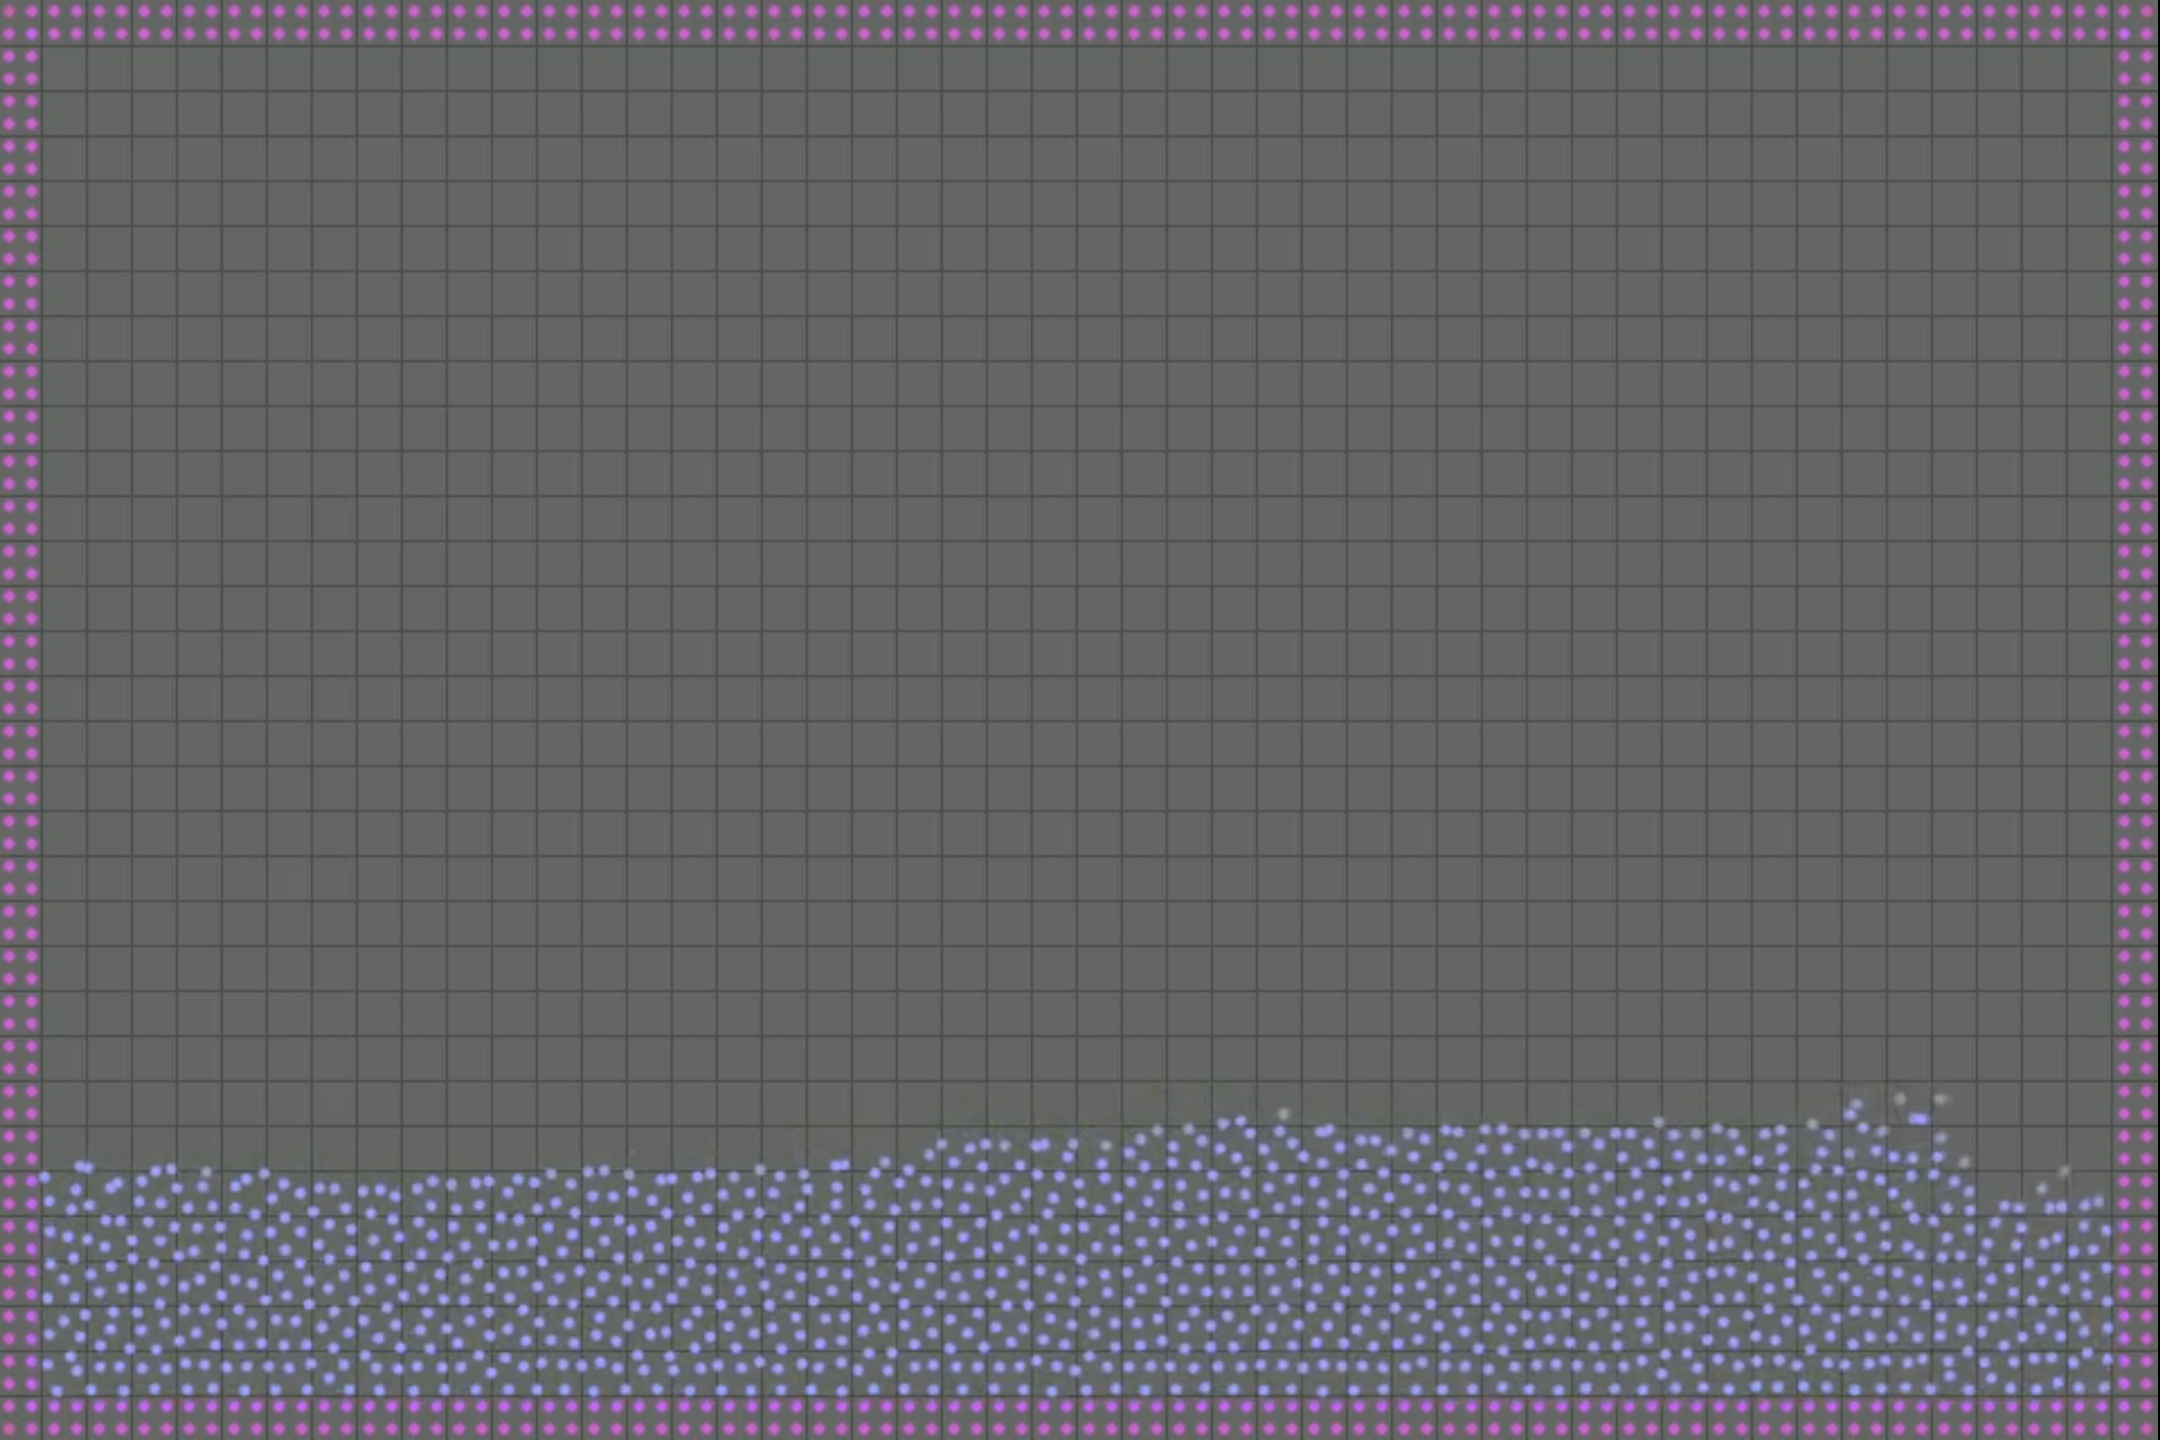
\includegraphics[width=\linewidth]{Boundary.png}
  \caption{Implementation of the new  boundary model.}
  \label{fig:boundary}
\end{figure}


As mentionned before, another implementation was done, with a more sophisticated boundary handling. The result can be seen on fig. \ref{fig:boundary}.

The qualitative result is not really obvious, though we may notice that the particles stay closer to the walls on resting positions, and avoid some small bouncing when they slide on the ground.

In theory, this method should be used to speed up the weighted Jacobi method, as the coefficients $\textbf{v}_{i}^{int}$, $\rho_i^{int}$, $\textbf{d}_{ii}$, $a_{ii}$, $\textbf{c}_i^l$ and $p_i^l$ do not need to be computed for wall particles.
In our case, only 1024 particles out of 1648 need to be computed in the method.
But after experimentation, it seems that the optimization is not that significant: the simulation is about 8\% faster. We suppose that it is due to the Jacobi method taking more step to converge. It is still a welcome improvement nevertheless.

\section{Conclusion}

While being notably slower than the original SPH method, the IISPH greatly improves the visual of the fluid simulation, especially for a liquid. It does not fix the density to an arbitrary value, but incites the particles to go in a configuration where the density is equal to this value.
The Jacobi method is not the quickest to resolve a system of equations, but is especially adapted for parallel computations, with a multi-threaded process, making this model faster than a majority of other incompressible SPH like PCISPH. It has a good balance between efficiency and quality of the simulation.

\bibliographystyle{ACM-Reference-Format}
\begin{thebibliography}{99}
\bibitem{IISPH} M. Ihmsen, J. Cornelis, B. Solenthaler, C. Horvath
and M. Teschner, 2014. Implicit incompressible SPH. IEEE
Transactions on Visualization and Computer Graphics 20, 426–
435.
\bibitem{SPH} J. Monaghan, “Smoothed Particle Hydrodynamics,” Ann. Rev.
Astronomy and Astrophysics, vol. 30, pp. 543-574, 1992.
\bibitem{WCSPH} M. Becker and M. Teschner, “Weakly Compressible SPH for Free
Surface Flows,” Proc. ACM SIGGRAPH/Eurographics Symp. Com-
puter Animation, pp. 209-217, 2007.
\bibitem{PCISPH} B. Solenthaler and R. Pajarola, “Predictive-Corrective Incompres-
sible SPH,” ACM Trans. Graphics, vol. 28, pp. 40:1-40:6, 2009.
\bibitem{ISPH} S. Shao and Y. Lo, “Incompressible SPH Method for Simulating
Newtonian and Non-Newtonian Flows with a Free Surface,”
Advances in Water Resources, vol. 26, no. 7, pp. 787-800, 2003
\bibitem{ISPHbis} M. Ellero, M. Serrano, and P. Espanol, “Incompressible Smoothed
Particle Hydrodynamics,” J. Computational Physics, vol. 226, no. 1,
pp. 1731-1752, 2007.
\bibitem{boundary} N. Akinci, M. Ihmsen, B. Solenthaler, G. Akinci, and M. Teschner,
“Versatile Rigid-Fluid Coupling for Incompressible SPH,” ACM
Trans. Graphics, vol. 30, no. 4, pp. 72:1-72:8, 2012.

\end{thebibliography}
\end{document}

